%برای شروع به فایل help.pdf رجوع کنید و فقط توجه داشته باشید کلاس VThesis.cls به کلاس SBU.cls، فایل اصلی از VThesis.tex به main.tex تغییر نام داده است.
\documentclass[oneside,a4paper,12pt,msc]{eceSBU}
% در این فایل، دستورها و تنظیمات مورد نیاز، آورده شده است.
%-------------------------------------------------------------------------------------------------------------------
\usepackage{pdfpages}
\usepackage[width=\linewidth,labelfont={small,bf,it},textfont={footnotesize,it}]{caption}
\usepackage[caption=false,font=footnotesize]{subfig}
\usepackage{verbatim}
\usepackage{amssymb,amsmath,amsthm}
%ایجاد فرورفتگی در اولین پاراگراف هر بخش
\usepackage{indentfirst}
%ایجاد فرورفتگی در اولین پاراگراف‌ها
\setlength{\parindent}{0.5cm}
% بسته‌ای برای تنطیم حاشیه‌های بالا، پایین، چپ و راست صفحه
\usepackage[top=30mm, bottom=30mm, left=30mm, right=30mm, headsep=0.5cm]{geometry}
% بسته‌‌ای برای ظاهر شدن شکل‌ها و تصاویر متن
\usepackage{graphicx}
\graphicspath{{./figs/}}
% بسته‌ای برای رسم کادر
\usepackage{framed} 
% بسته‌‌ای برای چاپ شدن خودکار تعداد صفحات در صفحه «معرفی پایان‌نامه» (در صورت استفاده)
\usepackage{lastpage}
% بسته‌‌هاایی برای ایجاد دیاگرام‌های مختلف
\usepackage{etoolbox}
\usepackage{pgfplots}
\usepackage{tikz}
\usepackage{tikzscale}
\usetikzlibrary{patterns}
\pgfplotsset{compat=1.9}

% بسته‌ و دستوراتی برای ایجاد لینک‌های رنگی با امکان جهش
\usepackage[linktocpage=true,colorlinks,pagebackref=true,linkcolor=blue,citecolor=magenta]{hyperref}
% چنانچه قصد پرینت گرفتن نوشته خود را دارید، خط بالا را غیرفعال و  از دستور زیر استفاده کنید چون در صورت استفاده از دستور زیر‌‌، 
% لینک‌ها به رنگ سیاه ظاهر خواهند شد که برای پرینت گرفتن، مناسب‌تر است
%\usepackage[pagebackref=false]{hyperref}
%بسته‌ی لازم برای مراجع در صورت به کار بردن natbib
%\usepackage[nonamebreak,square]{natbib}
%\usepackage[nonamebreak,square,numbers]{natbib}
%و اگرنه:
\usepackage{cite}

\usepackage{zref-perpage}
\zmakeperpage{footnote}
% بسته‌ لازم برای تنظیم سربرگ‌ها
\usepackage{fancyhdr}
% دستورات مربوط به ایجاد نمایه
\usepackage{makeidx}
\makeindex
%%%%%%%%%%%%%%%%%%%%%%%%%%
% فراخوانی بسته زی‌پرشین و تعریف قلم فارسی و انگلیسی
\usepackage{xepersian}
%\usepackage{bidiftnxtra}
\settextfont[Scale=1]{XB Niloofar}
%\setiranicfont[Scale=1]{PersianModern-Oblique}
%\setiranicfont[Scale=1]{B Nazanin}
\setlatintextfont[Scale=0.9]{FreeSans}
% چنانچه می‌خواهید اعداد در فرمول‌ها، انگلیسی باشد، خط زیر را غیرفعال کنید
%\setdigitfont{Yas}
\setdigitfont[Scale=.85]{Persian Modern}
%\setdigitfont[Scale=1.1]{XB Niloofar}
%\KashidaOn
%تنظیم فاصله‌ی خطوط و پاراگراف‌ها
\linespread{1.5}
\setlength{\parskip}{1ex plus 0.5ex minus 0.2ex}
%%%%%%%%%%%%%%%%%%%%%%%%%%
% تعریف قلم‌های فارسی و انگلیسی اضافی برای استفاده در بعضی از قسمت‌های متن
\defpersianfont\nastaliq[Scale=2]{IranNastaliq}
\defpersianfont\chapternumber[Scale=2]{IranNastaliq}
\defpersianfont\titr[Scale=1.8]{XB Niloofar}
\defpersianfont\dav[Scale=2.2]{B Davat}
%%%%%%%%%%%%%%%%%%%%%%%%%%
% دستوری برای حذف کلمه «چکیده»
\renewcommand{\abstractname}{}
% دستوری برای حذف کلمه «abstract»
\renewcommand{\latinabstract}{}
% دستوری برای تغییر نام کلمه «اثبات» به «برهان»
\renewcommand\proofname{\textbf{برهان}}
% دستوری برای تغییر نام کلمه «کتاب‌نامه» به «مراجع»
\renewcommand{\bibname}{مراجع}
%استفاده از کلمه‌ی نمودار به جای شکل
%\renewcommand{\figurename}{نمودار}
% دستوری برای تعریف واژه‌نامه انگلیسی به فارسی
\newcommand\persiangloss[2]{#1\dotfill\lr{#2}\\}
% دستوری برای تعریف واژه‌نامه فارسی به انگلیسی 
\newcommand\englishgloss[2]{#2\dotfill\lr{#1}\\}
%%%%%%%%%%%%%%%%%%%%%%%%%%
% تعریف و نحوه ظاهر شدن عنوان قضیه‌ها، تعریف‌ها، مثال‌ها و ...
\theoremstyle{definition}
\newtheorem{definition}{تعریف}[section]
%\newtheorem{deduct}[definition]{}
\newtheorem{theorem}[definition]{قضیه}
\newtheorem{lemma}[definition]{لم}
\newtheorem{proposition}[definition]{گزاره}
\newtheorem{corollary}[definition]{نتیجه}
\newtheorem{remark}[definition]{ملاحظه}
\newtheorem{example}[definition]{مثال}
%%%%%%%%%%%%%%%%%%%%%%%%%%
% تعریف دستورات جدید برای خلاصه نویسی و راحتی کار در هنگام تایپ فرمول‌های ریاضی
\newcommand{\mA}{\mathcal{A}}% مجموعه‌ی عامل‌ها
\newcommand{\mB}{\mathcal{B}}% زیرمجموعه‌ای از عامل‌ها
\newcommand{\mL}{\mathcal{L}}% زبان
\newcommand{\mF}{\mathcal{F}}% سیگما جبر
\newcommand{\mP}{\mathcal{P}}% تخصیص احتمالاتی
\newcommand{\mK}{\mathcal{K}}% منطق K
\newcommand{\mS}{\mathcal{S}}% منطق S5
\newcommand{\mbbP}{\mathbb{P}}% مجموعه‌ی گزاره‌های اتمی
\newcommand{\mbbQ}{\mathbb{Q}}% مجموعه‌ی اعداد گویا
\newcommand{\mbbM}{\mathbb{M}}% مجموعه‌ی مدل‌های شناختی احتمالاتی
\newcommand{\mbbK}{\mathbb{K}}% کلاس مدل‌های کریپکی
\newcommand{\mbbS}{\mathbb{S}}% کلاس مدل‌های شناختی
\newcommand{\mbP}{\mathbf{P}}% نماد تابعی احتمالاتی
\newcommand{\xra}{\xrightarrow}
\newcommand{\scr}{\scriptscriptstyle}
\newcommand{\bp}{\begin{proof}}
\newcommand{\ep}{\end{proof}}
%\newcommand{\close}{\begin{latin}\noindent $\square$ \end{latin}}
%%%%%%%%%%%%%%%%%%%%%%%%%%%%%%%%%%%%%%%%%%%
%تعریف اعداد لاتین برای زمانی که از اعداد فارسی در متن استفاده می‌کنیم
\def\0{\textrm{\lr{0}}}
\def\1{\textrm{\lr{1}}}
\def\2{\textrm{\lr{2}}}
\def\3{\textrm{\lr{3}}}
\def\4{\textrm{\lr{4}}}
\def\5{\textrm{\lr{5}}}
\def\6{\textrm{\lr{6}}}
\def\7{\textrm{\lr{7}}}
\def\8{\textrm{\lr{8}}}
\def\9{\textrm{\lr{9}}}
%%%%%%%%%%%%%%%%%%%%%%%%%%%%%%%%%%%%%%%%%%%
% براساس نسخه‌های از ۱.۲.۵ به بعد بسته‌ی bidi در توابع زیر باید توجه داشت:
% که l یعنی شروع نوشتار از ابتدای خط یا جعبه،
% و r یعنی شروع نوشتار از انتهای خط یا جعبه، 
% و s یعنی شروع نوشتار از وسط خط یا جعبه.
\newdimen\xleftright
\xleftright=\textwidth
\advance \xleftright by -10.5cm
\newcommand{\leftright}[3]{%
\noindent
\makebox[4 cm][r]{#1}
\makebox[\xleftright][s]{}
\makebox[5.5 cm][l]{#2}
\makebox[1 cm][l]{#3}%
}
\newcommand{\leftrightb}[2]{%
\noindent
\makebox[4 cm][r]{#1}
\makebox[\xleftright][s]{}
\makebox[6.5 cm][l]{#2}%
}
\newcommand{\semanticsa}[2]{%
\noindent
\makebox[4.3 cm][r]{#1}
\makebox[\xleftright][c]{اگر و فقط اگر}
\makebox[6.2 cm][l]{#2}%
}
\newcommand{\semanticsb}[2]{%
\noindent
\makebox[3.5 cm][l]{#1}
\makebox[\xleftright][c]{اگر و فقط اگر}
\makebox[7 cm][r]{#2}%
}
%%%%%%%%%%%%%%%%%%%%%%%%%%%%
% دستورهایی برای سفارشی کردن سربرگ صفحات
\csname@onesidetrue\endcsname
\fancypagestyle{main}{
\fancyhf{} 
\fancyhead[L]{\thepage}
}
\fancypagestyle{other}{
\fancyhf{} 
\fancyfoot[C]{\thepage}
}
% اگر می‌خواهید خط افقی بالای صفحه از بین برود:
\renewcommand{\headrulewidth}{0pt}
\appto\frontmatter{\pagestyle{other}}
\appto\mainmatter{\pagestyle{main}}

%%%%%%%%%%%%%%%%%%%%%%%%%%%%%
% دستورهایی برای سفارشی کردن صفحات اول فصل‌ها
\makeatletter
\newcommand\mycustomraggedright{%
 \if@RTL\raggedleft%
 \else\raggedright%
 \fi}
\def\@part[#1]#2{%
\ifnum \c@secnumdepth >-2\relax
\refstepcounter{part}%
\addcontentsline{toc}{part}{\thepart\hspace{1em}#1}%
\else
\addcontentsline{toc}{part}{#1}%
\fi
\markboth{}{}%
{\centering
\interlinepenalty \@M
\ifnum \c@secnumdepth >-2\relax
 \huge\bfseries \partname\nobreakspace\thepart
\par
%\vskip 20\p@
\fi
\Huge\bfseries #2\par}%
\@endpart}
\def\@makechapterhead#1{%
\vspace*{280\p@}%
{\parindent \z@ \mycustomraggedright %\@mycustomfont
\ifnum \c@secnumdepth >\m@ne
\if@mainmatter
\renewcommand{\thechapter}{\nastaliq\tartibi{chapter}}
%\centering
\hspace{2cm}\nastaliq \bfseries \@chapapp\space {\chapternumber\thechapter}
\par\nobreak
%\vskip 20\p@
\fi
\fi
\centering
\interlinepenalty\@M 
\thispagestyle{empty}
\titr \bfseries #1\par\clearpage
}}

 \def\abj@num@i#1{%
   \ifcase#1\or الف\or ب\or ج\or د%
            \or ه‍\or و\or ز\or ح\or ط\fi
   \ifnum#1=\z@\abjad@zero\fi}
   
\renewcommand*{\thesubfigure}{\harfi{subfigure}} 
\providecommand\thefigsubsep{.}
\def\p@subfigure{\@nameuse{thefigure}\thefigsubsep}
\makeatother
%دستور عددگذاری صحیح معادله‌ها
\renewcommand*{\theequation}{\arabic{equation}-\thechapter}
%دستور عددگذاری صحیح شماره الگوریتم‌ها (در صورت استفاده
%\renewcommand*{\thealgorithm}{(\arabic{algorithm}-\thechapter)}
%دستور برای این که نام فهرست شکل‌ها به درستی ظاهر شود.
\renewcommand\listfigurename{فهرست شکل‌ها}

\begin{document}
\frontmatter
%%%%%%%%%%%%%%%%%%%%%%%%%%%%%%%%%%%%%%%%%
%صفحه‌ی بسم الله
%\thispagestyle{empty}
%\centerline{{\includegraphics[width=9 cm]{*}}}
%\newpage
%\thispagestyle{empty}
%\clearpage
%~~~
%%%%%%%%%%%%%%%%%%%%%%%%%%%%%%%%%%%%%%%%%
\clearpage
\pagenumbering{adadi}
\newpage\null\thispagestyle{empty}\newpage
% در این فایل، عنوان پایان‌نامه، مشخصات خود، متن تقدیمی‌، ستایش، سپاس‌گزاری و چکیده پایان‌نامه را به فارسی، وارد کنید.
% توجه داشته باشید که جدول حاوی مشخصات پایان‌نامه/رساله و همچنین، مشخصات داخل آن، به طور خودکار، درج می‌شود.
%%%%%%%%%%%%%%%%%%%%%%%%%%%%%%%%%%%%
% دانشگاه خود را وارد کنید
\university{شهید بهشتی}
% دانشکده، آموزشکده و یا پژوهشکده  خود را وارد کنید
\faculty{علوم و مهندسی کامپیوتر}
% گروه آموزشی خود را وارد کنید
\degree {کارشناسی ارشد} 
% گروه آموزشی خود را وارد کنید
%\subject{ مهندسی کامپیوتر}
% گرایش خود را وارد کنید
%\renewcommand{\subjec}{def}
\field{مهندسی کامپیوتر - گرایش هوش مصنوعی}
% عنوان پایان‌نامه را وارد کنید
\title{ارائه‌ی روشی بدون مرجع و کارا برای تخمین زدن کیفیت تصاویر}
% نام استاد(ان) راهنما را وارد کنید
\firstsupervisor{دکتر محسن ابراهیمی مقدم}
%\secondsupervisor{استاد راهنمای دوم}
% نام استاد(دان) مشاور را وارد کنید. چنانچه استاد مشاور ندارید، دستور پایین را غیرفعال کنید.
%\firstadvisor{استاد مشاور اول}
%\secondadvisor{استاد مشاور دوم}
% نام پژوهشگر را وارد کنید
\name{محمد مسعود}
% نام خانوادگی پژوهشگر را وارد کنید
\surname{مسائلی}
% تاریخ پایان‌نامه را وارد کنید
\thesisdate{1394}
% کلمات کلیدی پایان‌نامه را وارد کنید
\keywords{ارزیابی کیفیت تصویر، زیبایی شناسی بصری، ارزیابی بدون مرجع کیفیت تصویر}
% چکیده پایان‌نامه را وارد کنید
\fa-abstract{\noindent
با رشد روز افزون تکنولوژی و افزایش توانایی پردازش ماشین، شاهد رشد چشم گیر پردازش تصویر دیجیتال هستیم. یکی از مسائلی که در مسیر تصویربرداری الی نمایش آن پیش می‌آید، این است که ممکن است در این مسیر تصویر به هر نحوی دچار خرابی یا دستخوش تغییراتی ناخوشایند شود. اگر بتوان پیش از نمایش تصویر، ایراد پیش‌آمده بر روی آن را شناسایی کرد، حل کردن تخریب آسان شده و کاربر می‌تواند به تصویری سالم و چشم‌نواز دست یابد.\\
در این پایان‌نامه، حوزه‌ی ارزیابی بدون مرجع کیفیت تصویر را زیر ذره‌بین گذاشته و با استفاده از مفاهیم و معیارهای زیبایی شناسی، روش‌های به روز آن را غنی کردیم. برای این کار، معیارهای زیبایی شناسی موجود در مبحث «هنرهای فرگشتی» و «ارزیابی کیفیت عکس» را به کار بسته، با دادن تغییرات و گاهی پیاده سازی کاملاً نوآورانه، یک دسته ویژگی ایجاد نمودیم. سپس ثابت شد که قرار دادن این دسته ویژگی در کنار ویژگی‌های روش‌های به روز دنیا، باعث بهبود چشمگیر دقت آن‌ها می‌شود. در نهایت، یکی از دقیق‌ترین شیوه‌های روز ارزیابی بدون مرجع کیفیت تصویر را به کار بستیم و با افزودن ویژگی‌های زیبایی شناسی پیشنهاد شده، یک روش دقیق و کارا برای این حوزه ارائه دادیم. 
}


%%%%%%%%%%%%%%%%%%%%%%%%%%%%%%%%%%%%%%%%%%%%%%%%%%%%%%%%%%%%%
\ \\ \\ \\ \\ \\ \\ \\ \\ \\
{
\vspace*{3cm}

\centering{\nastaliq''این قوی‌ترین گونه نیست که بقا پیدا می‌کند، باهوش‌ترین هم نیست؛ گونه‌ای بقا پیدا می‌کند که بیشترین سازگاری در مقابل تغییرات را داشته باشد``}
\begin{flushleft}
-چارلز داروین
\end{flushleft}
\begin{comment}
\vspace*{2cm}

\selectfont\centering\lr{``It is not the strongest of the species that survive, nor the most intelligent, but the one most responsive to change.''}
\begin{flushright}
\lr{-Charles Darwin}
\end{flushright}
\end{comment}
}


\newpage
\thispagestyle{empty}
\vtitle


\includepdf[pages={4}]{formsAndPapers/forms.pdf}
\newpage
%\thispagestyle{empty}
% سپاس‌گزاری
{\nastaliq
سپاس‌گزاری...
}
\\[2cm]
در آغاز وظیفه‌ی خود می‌دانم از راهنمایی‌ها و زحمات آقای دکتر ابراهیمی مقدم در به ثمر رسیدن این پایان‌نامه قدردانی نمایم.
\\
همچنین جا دارد که تشکری ویژه داشته باشم از دوست عزیزم «محسن جنادله» که با حوصله و انتقادهای به جا مرا در انجام این پایان نامه و نوشتن مقالات مربوطه یاری نمود.
\\
و نیز سپاسگزارم از تمامی اساتیدی که بر پیشرفت علمی اینجانب تأثیرگذار بودند و دکتر علی ذاکرالحسینی که ناخواسته باعث شدند صبر و شکیبایی را بیاموزم.
\\
در آخر لازم است از آقایان وفا خلیقی (پدیدآورنده‌ی \XePersian)، محمود امین‌طوسی، هادی صفی‌اقدم، وحید دامن‌افشان و دیگر دوستانی که در سایت وزین \href{www.parsilatex.com}{\lr{www.parsilatex.com}} به راهنمایی کاربران \TeX فارسی می‌پردازند قدردانی نمایم.
\\
و بوسه می‌زنم بر دستان پدر و مادر عزیزم که با محبت‌های نامتناهی زندگی مرا به پیروزی روزافزون متمایل می‌کنند.

% با استفاده از دستور زیر، امضای شما، به طور خودکار، درج می‌شود
\signature 
%
\includepdf[pages={6}]{formsAndPapers/forms.pdf}
\ \\ \\ \\ \\ \\ \\ \\ \\ \\
{\dav
\begin{center}
كلية حقوق اعم از چاپ و تكثير، نسخه برداری ، ترجمه، اقتباس و ... از اين پايان نامه براي دانشگاه شهيد بهشتي محفوظ است.
 نقل  مطالب با ذكر مأخذ آزاد است.
\end{center}
}


\includepdf[pages={8}]{formsAndPapers/forms.pdf}
\begin{comment}
 % پایان‌نامه خود را تقدیم کنید!
\begin{acknowledgementpage}

\vspace{4cm}

{\nastaliq
{\Large
 تقدیم به آنکس که بداند و بداند که بداند 
\vspace{1.5cm}

\newdimen\xa
\xa=\textwidth
\advance \xa by -11cm
\hspace{\xa}
و آنکس که نداند و بداند که نداند و بخواهد که بداند
}}
\end{acknowledgementpage}
\newpage
\thispagestyle{empty}
\clearpage
~~~
\end{comment}

%\include{preface}
\tableofcontents
\newpage
\phantomsection
\addcontentsline{toc}{chapter}{فهرست شکل‌ها}
\listoffigures
\newpage
\phantomsection
\addcontentsline{toc}{chapter}{فهرست جداول}
\listoftables
%\clearpage{\pagestyle{empty}\cleardoublepage}
%\clearpage
%\vspace{5cm}
%\phantomsection
%\addcontentsline{toc}{chapter}{چکیده}
\chapter*{چکیده}\markboth{چکیده}{چکیده}
%\abstractview
%\begin{comment}
%\vspace*{1cm}
با رشد روز افزون فناوری و افزایش توانایی پردازش ماشین، شاهد رشد چشمگیر پردازش تصویر دیجیتال هستیم. یکی از مسائلی که در مسیر تصویربرداری تا نمایش آن پیش می‌آید، این است که ممکن است در این مسیر تصویر به هر نحوی دچار خرابی یا دستخوش تغییراتی ناخوشایند شود. اگر بتوان پیش از نمایش تصویر، ایراد پیش‌آمده بر روی آن را شناسایی کرد، برطرف کردن تخریب آسان شده و کاربر می‌تواند به تصویری سالم و چشم‌نواز دست یابد.

در این پایان‌نامه، حوزه‌ی ارزیابی بدون مرجع کیفیت تصویر را زیر ذره‌بین گذاشته و با استفاده از مفاهیم و معیارهای زیبایی شناسی، روش‌های به روز آن را غنی کردیم. برای این کار، معیارهای زیبایی شناسی موجود در مباحث «هنرهای فرگشتی» و «ارزیابی کیفیت عکس» را به کار بسته، با دادن تغییرات و گاهی پیاده سازی کاملاً نوآورانه، یک دسته ویژگی ایجاد نمودیم. سپس ثابت شد که قرار دادن این دسته ویژگی در کنار ویژگی‌های روش‌های به روز دنیا، باعث بهبود چشمگیر دقت آن‌ها می‌شود. آزمایش‌های متعددی با استفاده از پایگاه‌های داده‌ی رایج این بحث اعم از پایگاه داده‌ی \متن‌لاتین{LIVE}، \متن‌لاتین{CSIQ} و \متن‌لاتین{TID2013} صورت گرفت و نشان داده شد که بهترین روش‌های حال حاضر ارزیابی بدون مرجع کیفیت تصویر در کنار ویژگی‌های زیبایی شناسی بهتر از گذشته عمل می‌کنند. این بهتر عمل کردن به این معنی است که همبستگی نمرات ذهنی که انسان‌ها به تصاویر مختلف پایگاه‌های داده نسبت داده‌اند با خروجی روش‌ها بیشتر شده و خطای ارزیابی کیفیت تصویر توسط همه‌ی این روش‌های بدون مرجع ارزیابی کیفیت تصویر پس از افزودن ویژگی‌های زیبایی شناسی کاهش یافته است. نتایج در غالب «همبستگی خطی اسپیرمن»، «همبستگی رتبه‌ای پیرسون»، «همبستگی رتبه‌ای کندال» و همچنین «مجذور میانگین مربعات خطا» و «میانگین مطلق خطا» ارائه شده است و به ازای همه‌ی این محک‌ها شاهد بهبود در عملکرد ارزیابی بدون مرجع کیفیت تصویر هستیم؛ نتیجه‌ی این بهبود این است که نمرات عینی کیفیت که حاصل از پردازش‌های مختلف بر روی تصاویر است به نمرات ذهنی که نظر مستقیم انسانی است نزدیک‌تر می‌شود. با توجه به این که غالباً کاربر نهایی سیستم‌های ارزیابی کیفیت تصویر انسان است، نزدیک شدن هر چه بیشتر خروجی روش‌های ارزیابی کیفیت تصویر به نمرات ذهنی، آرزوی دیرین انسان در این شاخه بوده است.

در نهایت، یکی از دقیق‌ترین شیوه‌های روز ارزیابی بدون مرجع کیفیت تصویر را به کار بستیم و با افزودن ویژگی‌های زیبایی شناسی پیشنهاد شده، یک روش دقیق و کارا برای این حوزه ارائه دادیم. این روش دقیق، کارایی بالاتری نسبت به بهترین روش‌های حال حاضر ارزیابی بدون مرجع کیفیت تصویر از خود نشان می‌دهد.
\\ \\
\textbf{کلمات کلیدی:} ارزیابی کیفیت تصویر، زیبایی شناسی بصری، ارزیابی بدون مرجع کیفیت تصویر

%\end{comment}

\mainmatter
\فصل{مقدمات}
\برچسب{فصل:مقدمه}
\قسمت{آغاز مثلاً}
این فصل به مقدمات پایان نامه اختصاص دارد. ابتدا مسأله‌ی ارزیابی کیفیت تصویر(\متن‌لاتین{IQA}\پانویس{Image Quality Assessment}) را تعریف کرده، سپس به کاربردهای آن اشاره می‌کنیم. پس از آن رویکرد نویی که این پایان نامه به مسئله‌ی \متن‌لاتین{IQA} دارد را مورد بررسی قرار داده و نهایتاً ساختار کلی متنی که پیش رو است را از نظر می‌گذرانیم.

\begin{comment}
\begin{figure}[ht]
  \centering
  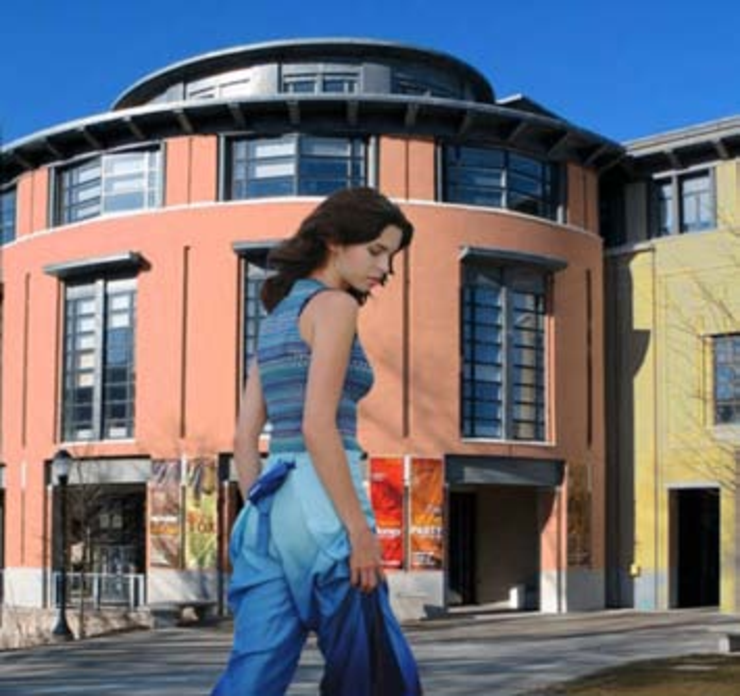
\includegraphics[width=0.9\linewidth]{harmonized.pdf}
  \شرح{شرح \متن‌لاتین{harmonized.pdf} \مرجع{someCitation}}
  \label{شکل:دسته‌های‌IQA}
\end{figure}
\end{comment}
\قسمت{ساختار پایان‌نامه}

\فصل{مرور روش‌های مرتبط}
\برچسب{کارهای‌گذشته}

\فصل{روش پیشنهادی}
\برچسب{فصل:شیوه‌تحقیق}

\فصل{نتایج تحقیق}
\برچسب{فصل:یافته‌های‌تحقیق}

\فصل{نتیجه‌گیری و پیشنهاد کارهای آتی}
\برچسب{فصل:نتیجه‌گیری}


\makeatletter
\def\@harfi#1{\ifcase#1\or الف\or ب\or پ\or ت\or ث\or
ج\or چ\or ح\or خ\or د\or ذ\or ر\or ز\or ژ\or س\or ش\or ص\or ض\or ط\or ظ\or ع\or غ\or
ف\or ق\or ک\or گ\or ل\or م\or ن\or و\or ه\or ی\else\@ctrerr\fi}
\def\@makechapterhead#1{
\vspace*{280\p@}
{\parindent \z@ \mycustomraggedright
\ifnum \c@secnumdepth >\m@ne
\if@mainmatter
\renewcommand{\thechapter}{\nastaliq\harfi{chapter}}
\hspace{2cm}\nastaliq \bfseries \@chapapp\space {\chapternumber\thechapter}
\par\nobreak
\fi
\fi
\centering
\interlinepenalty\@M 
\thispagestyle{empty}
\titr \bfseries #1\par\clearpage
}}
\makeatother

\newpage
\appendix
\phantomsection
\addcontentsline{toc}{chapter}{\rl{پیوست الف~~~~این پیوست اول است}}
\addtocontents{toc}{\protect\setcounter{tocdepth}{-1}}
\فصل{این پیوست اول است}
\برچسب{فصل:پیوست اول}

\addtocontents{toc}{\protect\setcounter{tocdepth}{1}}

{\small
\newpage
\phantomsection
\addcontentsline{toc}{chapter}{\rl{مراجع}}
 \bibliographystyle{ieeetr-fa} 
\bibliography{myReferences} 
}
\backmatter

% در این فایل، عنوان پایان‌نامه، مشخصات خود و چکیده پایان‌نامه را به انگلیسی، وارد کنید.
% توجه داشته باشید که جدول حاوی مشخصات پایان‌نامه/رساله، به طور خودکار، رسم می‌شود.
%%%%%%%%%%%%%%%%%%%%%%%%%%%%%%%%%%%%
\baselineskip=.6cm
\begin{latin}
\begin{comment}
\latinuniversity{Shahid Beheshti University}
\latinfaculty{Faculty of Computer Science and Engineering}
\latindegree{M.Sc of Artificial Intelligence}
%group:
%\latinsubject{Department of Mathematics}
\latinfield{Artificial Intelligence}
\latintitle{An Efficient Method for Blind Image Quality Assessment}
\firstlatinsupervisor{Dr. Mohsen Ebrahimi Moghaddam}
%\secondlatinsupervisor{Second Supervisor}
%\firstlatinadvisor{First Advisor}
%\secondlatinadvisor{Second Advisor}
\latinname{Mohammad Masood}
\latinsurname{Masaeli}
\latinthesisdate{2015}
\latinkeywords{Blind image quality assessment, Computational  image aesthetic, Statistical model}
\en-abstract{\noindent
The main goal of image quality assessment methods is imitation of human perceptual image quality judgments, therefore, the correlation between objective scores of these methods with corresponding human perceptual scores is considered as their performance. Human judgment of image quality implicitly comprehends many factors which some are ignored by current Blind Image Quality Assessment (BIQA) methods. They only consider content independent factors like sharpness, noise, dynamic range, contrast, distortion, exposure accuracy and blur, while the human judgment on image quality also considers image content and aesthetics. This results in different opinion scores for images affected by same distortions with same severity. In order to simulate human judgments in this thesis, we proposed an approach to enrich features of existing BIQA methods by a bag of aesthetic based features. The proposed features are tested on benchmark databases and showed capability of making improvements on state-of-the-art methods' performances. Finally a new method for BIQA implemented which involves one of the best state-of-the-art methods enriched by aesthetic features and by intensive experiments, proved to be able to beat all other methods in accuracy.
}
\latinvtitle
\end{comment}
\newpage\thispagestyle{empty}
\chapter*{Abstract:}
\vspace*{3cm}

{\noindent
The main goal of image quality assessment methods is imitation of human perceptual image quality judgments, therefore, the correlation between objective scores of these methods with corresponding human perceptual scores is considered as their performance. Human judgment of image quality implicitly comprehends many factors which some are ignored by current Blind Image Quality Assessment (BIQA) methods. They only consider content independent factors like sharpness, noise, dynamic range, contrast, distortion, exposure accuracy and blur, while the human judgment on image quality also considers image content and aesthetics. This results in different opinion scores for images affected by same distortions with same severity. In order to simulate human judgments in this thesis, we proposed an approach to enrich features of existing BIQA methods by a bag of aesthetic based features. The proposed features are tested on well-known benchmark databases such as LIVE, CSIQ, and TID2013 and showed capability of making improvements on state-of-the-art methods' performances. In particular, we compared the state-of-the-art methods with their enriched versions via linear Pearson's correaltion coefficient, ranked order Spearman and Kendall's correlatio coefficient and RMSE and mean absolute error (MAE). All the results showed accuracy of these methods improved by adding the aesthetic features which means the objective quality scores predicted by the methods got closer to human subjective scores.
\\
Finally a new method for BIQA implemented which involves one of the best state-of-the-art methods enriched by aesthetic features and by intensive experiments, proved to be able to beat all other methods in accuracy.
}
\newpage

\includepdf[pages={10}]{formsAndPapers/forms.pdf}
\end{latin}

\label{LastPage}
\end{document}
